\chapter{Các hệ thống liên quan trong thực tế}

\section{Các nhà cung cấp dịch vụ Mạng xã hội và truyền thông xã hội đang từng bước hỗ trợ kinh doanh trực tuyến}
\subsection{Facebook với Shopping Marketplace}

Facebook là mạng xã hội rất phổ biến, cho phép người dùng đăng tải ảnh, video, chia sẻ những status cảm xúc, gửi các thông điệp tới bạn bè. Tuy nhiên trong những năm gần đây nhiều người đã sử dụng Facebook để kết nối theo cách khác: mua và bán. Hoạt động này bắt đầu trong Facebook Groups và đã phát triển đáng kể. Hơn 450 triệu người đến tham quan mua và bán các nhóm mỗi tháng - từ các gia đình trong một khu phố địa phương cho tới quy mô toàn thế giới.

\begin{figure}[H]
	\centering
	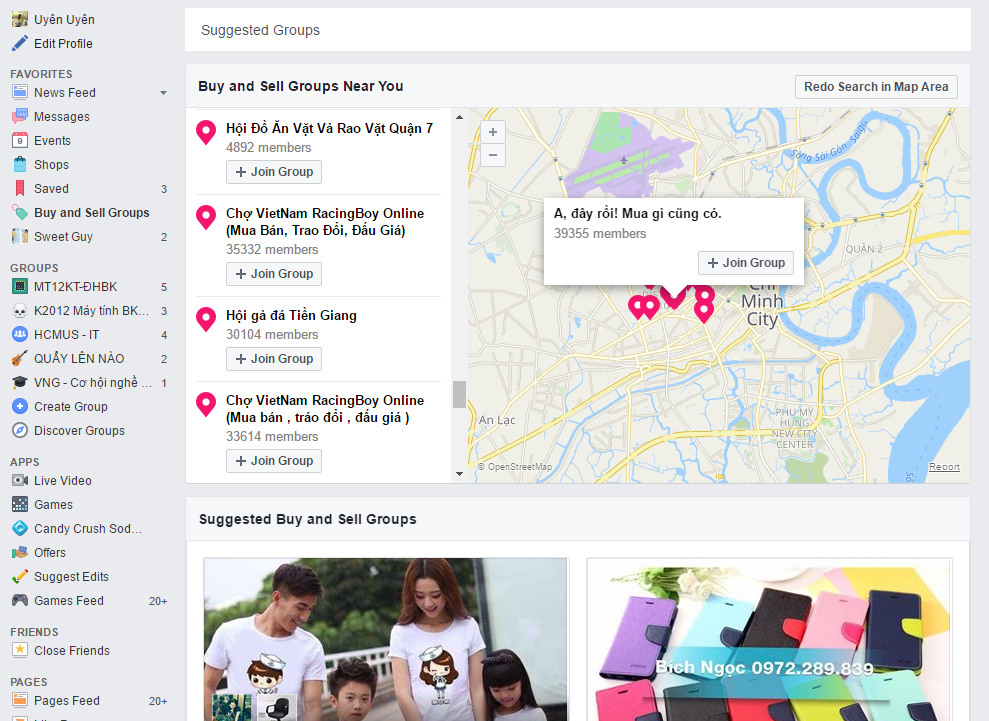
\includegraphics[scale=.5]{img/fb-group-buy.PNG} 
	\caption{Facebook Groups - Buy and Sell Groups}
\end{figure}

Nhằm hỗ trợ cho sự tương tác mới này, Facebook đã cho ra đời Facebook Marketplace, nơi người dùng có thể lên danh sách những thứ họ có hoặc mong muốn trong một phạm vi kết nối ("[...] to list what you have and what you want within your group of friends, networks, or other networks. Beyond its use for classified listings, you can use Marketplace to get a sense of everything available or desired within your networks."\cite{facebooknote1}).

Một số hình ảnh của Facebook Marketplace:

\begin{figure}[H]
	\centering
	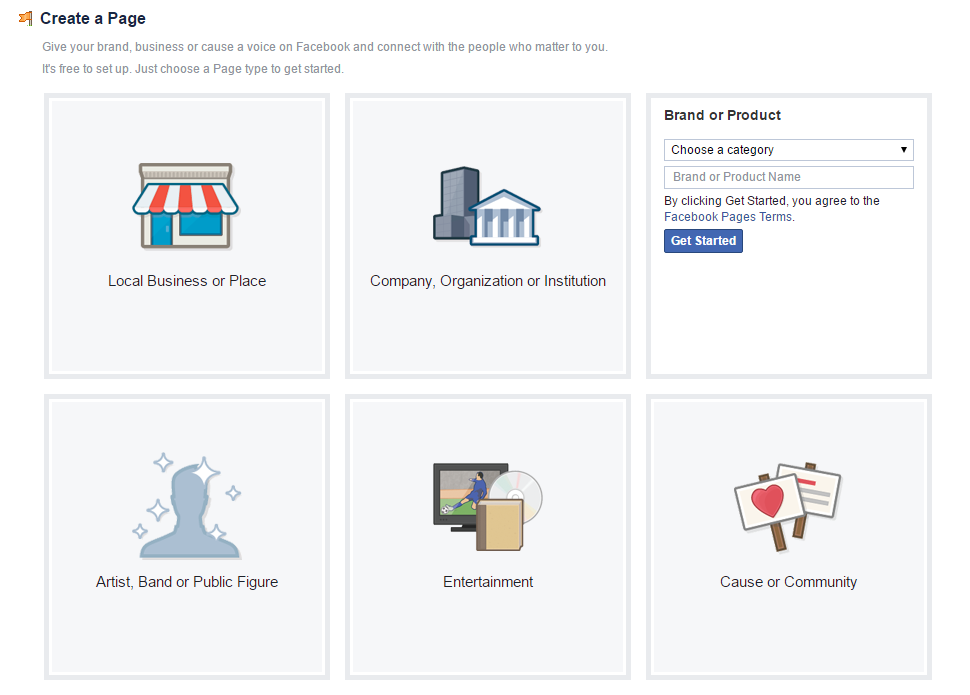
\includegraphics[scale=.5]{img/fb-create-page.PNG} 
	\caption{Tạo một Page trong Facebook Marketplace}
\end{figure}

\begin{figure}[H]
	\centering
	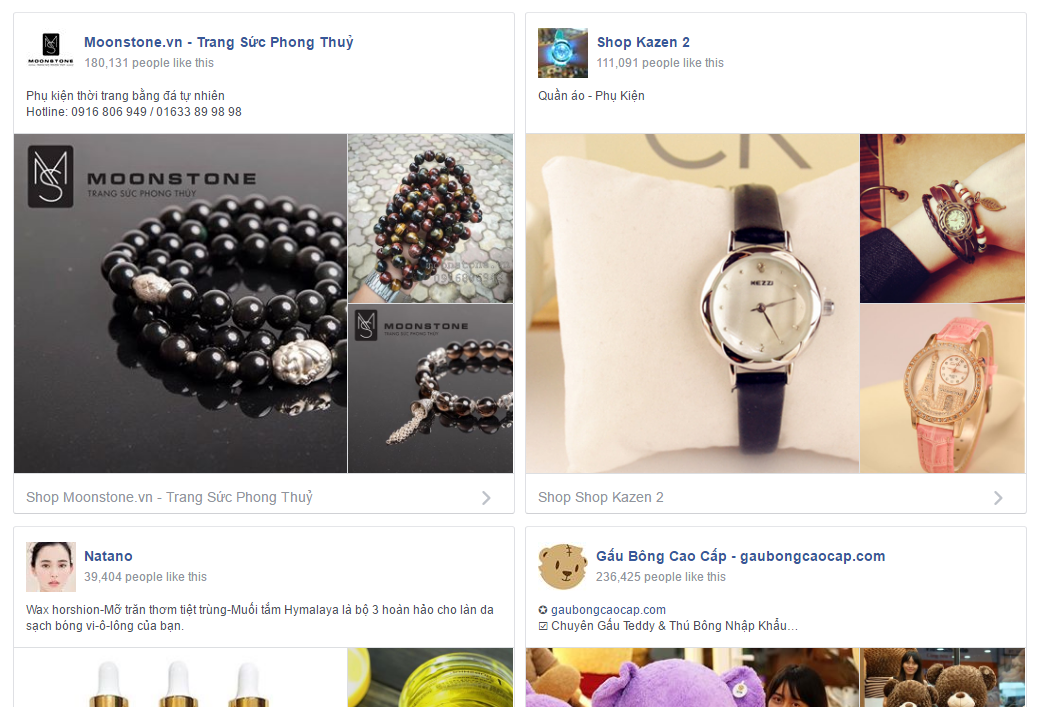
\includegraphics[scale=.5]{img/fb-shop.PNG} 
	\caption{Các Pages được trình bày tại trang chính của Marketplace}
\end{figure}

\begin{figure}[H]
	\centering
	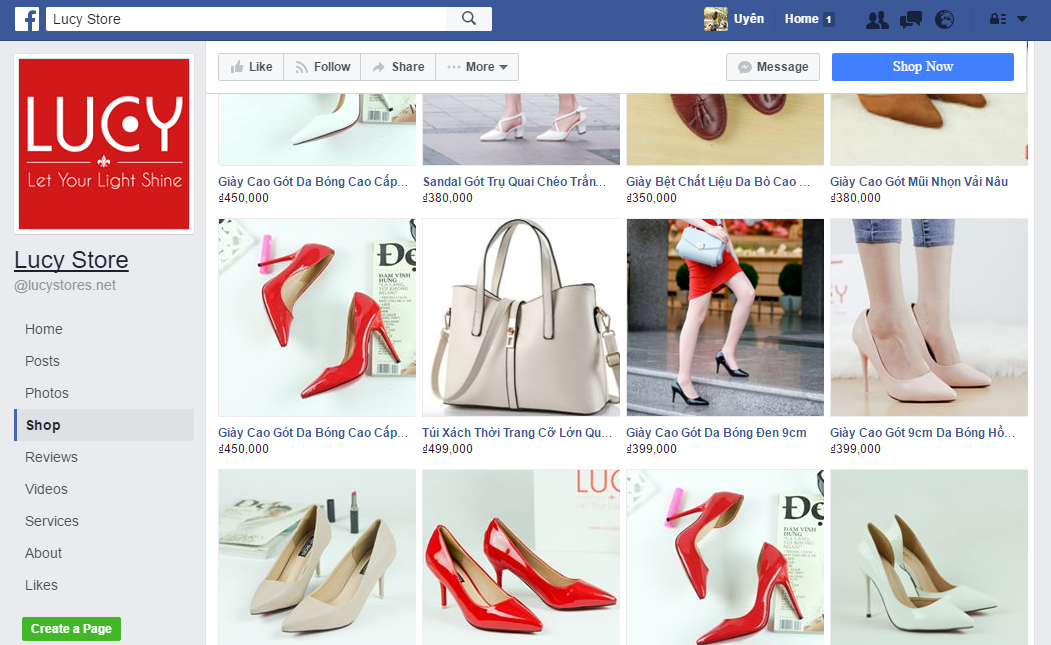
\includegraphics[scale=.5]{img/fb-in-store.PNG} 
	\caption{Giao diện trong Page được thiết kế như một cửa hàng trực tuyến}
\end{figure}

Từ những thông tin trên, ta thấy mạng xã hội này đang từng bước đưa khái niệm thương mại điện tử vào trong hệ thống của họ. Tuy nhiên, việc mua bán này chỉ đang dừng lại ở mức độ giao diện, trưng bày chứ chưa hỗ trợ người dùng trong toàn bộ quá trình mua, bán.

\subsection{Pinterest với "Buyable Pins"}
Khởi đầu với một trang web chia sẻ hình ảnh trực tuyến được biết đến như là "danh mục ý tưỏng" ("catalog of ideas" - CEO Ben Silbermann) hơn là một mạng xã hội. Tuy nhiên, vào tháng 6/2015 Pinterest tuyên bố phát hành những "Buyable Pins", là những "Pin" được tích hợp nút "Buy it" bên cạnh nút "Pin it" thông thường. Những "Pin" này được tạo bởi các doanh nghiệp để quảng bá sản phẩm của họ thông qua Pinboards. Người dùng cũng có thể thấy giá của các mặt hàng, và được hỗ trợ để thanh toán (mua) ngay trên Pinterest thông qua Apple Pay hoặc Credit Cart. 

\begin{figure}[H]
	\centering
	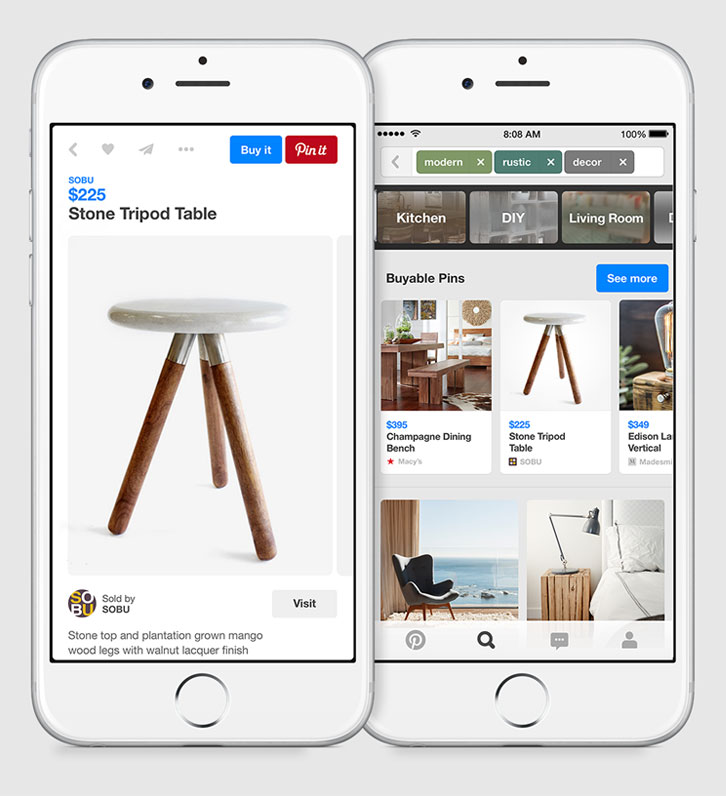
\includegraphics[scale=.4]{img/pin-buypins.jpg} 
	\caption{Buyable pins trên Iphone}
\end{figure}

Với lợi thế về khả năng chia sẻ của Pinterest, khi người mua "re-pin" một thứ mà họ thích, nó sẽ được lan truyền và tiếp thị rộng rãi như virus, lan sang các nhóm khác nhau. 

Dù được quảng cáo với nhiều ưu điểm tuyệt vời, mua bán trên Pinterest vẫn còn những hạn chế. Những người chủ của Pinterest không muốn sản phẩm của mình là một mạng xã hội mà quyết giữ nó theo quan điểm ban đầu và luôn duy trì quan điểm thận trọng đối với sự phát triển mới\cite{AllYouNeedtoKnowAboutPinterestBuyablePins}, hiện tại khả năng mua bán của nó có được là do sự liên kết với những nền tảng thương mại điện tử khác một cách hạn chế bao gồm BigCommerce, Demandware, Magento và Shopify, và hiện chỉ hoạt động tại Mỹ. Do đó, việc mua bán và thanh toán trên Pinterest gặp nhiều khó khăn.

(lợi thế của sự hợp tác giữa shopify với pinterest)

(nhận xét chung)
\section{Các trang thương mại điện tử đang từng bước cải thiện sự tương tác thành viên}

\subsection{Chợ điện tử Alibaba với }

\subsection{Amazon}

Mục đích của việc tích hợp tính năng xã hội trong các ứng dụng thương mại điện tử là để động viên người tiêu dùng truy cập ứng dụng thường xuyên hơn và trong thời gian dài của thời gian, với hy vọng chuyển đổi lần vào bán hàng.

